\chapter{\RU{Условные переходы}\EN{Conditional jumps}}
\label{sec:Jcc}
\index{\CLanguageElements!if}

% sections
\section{\RU{Простой пример}\EN{Simple example}}

\lstinputlisting{patterns/07_jcc/simple/ex.c}

% subsections
\subsection{x86}

\subsubsection{x86 + MSVC}

\RU{Имеем в итоге функцию \TT{f\_signed()}:}\EN{Here is how the \TT{f\_signed()} function looks like:}

\lstinputlisting[caption=\NonOptimizing MSVC 2010]{patterns/07_jcc/simple/signed_MSVC.asm}

\index{x86!\Instructions!JLE}
\RU{Первая инструкция \JLE значит}
\EN{The first instruction, \JLE, stands for} \IT{Jump if Less or Equal}. 
\RU{Если второй операнд больше первого или 
равен ему, произойдет переход туда, где будет следующая проверка.}
\EN{In other words, if the second operand is 
larger or equal to the first one, the control flow will be passed to the specified in the instruction address or label.}
\RU{А если это условие не срабатывает (то есть второй операнд меньше первого), то перехода не будет, 
и сработает первый \printf.}
\EN{If this condition does not trigger because the second operand is smaller than the first one, the control flow would not be altered and the first \printf would be executed.}
\index{x86!\Instructions!JNE}
\RU{Вторая проверка это}\EN{The second check is} \JNE: \IT{Jump if Not Equal}.
\RU{Переход не произойдет, если операнды равны}\EN{The control flow will not change if the operands are 
equal}.

\index{x86!\Instructions!JGE}
\RU{Третья проверка}\EN{The third check is} \JGE: \IT{Jump if Greater or Equal}\EMDASH{}\RU{переход 
если первый операнд больше второго или равен ему}\EN{jump if the first operand is larger than 
the second or if they are equal}.
\RU{Кстати, если все три условных перехода сработают, ни один \printf не вызовется. 
Но без внешнего вмешательства это невозможно.}
\EN{So, if all three conditional jumps are triggered, none of the \printf calls would be executed whatsoever. 
This is impossible without special intervention.}

\EN{Now let's take a look at the \TT{f\_unsigned()} function.}
\EN{The}\RU{Функция} \TT{f\_unsigned()} \RU{точно такая же, за тем исключением, что используются инструкции 
\JBE и \JAE вместо \JLE и \JGE:}
\EN{function is the same as \TT{f\_signed()}, with the exception that the \JBE and \JAE instructions
are used instead of \JLE and \JGE, as follows:}

\lstinputlisting[caption=GCC]{patterns/07_jcc/simple/unsigned_MSVC.asm}

\index{x86!\Instructions!JBE}
\index{x86!\Instructions!JAE}
\RU{Здесь всё то же самое, только инструкции условных переходов немного другие:}
\EN{As already mentioned, the branch instructions are different:}
\JBE\EMDASH{}\IT{Jump if Below or Equal} \AndENRU \JAE\EMDASH{}\IT{Jump if Above or Equal}.
\RU{Эти инструкции}\EN{These instructions} (\JA/\JAE/\JB/\JBE) 
\RU{отличаются от}\EN{differ from} \JG/\JGE/\JL/\JLE \RU{тем, что работают с беззнаковыми переменными.}
\EN{in the fact that they work with unsigned numbers.}

\index{x86!\Instructions!JA}
\index{x86!\Instructions!JB}
\index{x86!\Instructions!JG}
\index{x86!\Instructions!JL}
\index{Signed numbers}
\RU{Отступление: смотрите также секцию о представлении знака в числах}
\EN{See also the section about signed number representations}~(\myref{sec:signednumbers}).
\RU{Таким образом, увидев где используется \JG/\JL вместо \JA/\JB и наоборот, 
можно сказать почти уверенно насчет того, 
является ли тип переменной знаковым (signed) или беззнаковым (unsigned).}
\EN{That is why if we see \JG/\JL in use instead of \JA/\JB or vice-versa, 
we can be almost sure that the variables are signed or unsigned, respectively.}

\RU{Далее функция \main, где ничего нового для нас нет:}
\EN{Here is also the \main function, where there is nothing much new to us:}

\lstinputlisting[caption=\main]{patterns/07_jcc/simple/main_MSVC.asm}

\ifdefined\IncludeOlly
\clearpage
\subsubsection{x86 + MSVC + \olly}
\index{\olly}
\index{x86!\Registers!\Flags}

\RU{Если попробовать этот пример в \olly, можно увидеть, как выставляются флаги}\EN{We
can see how flags are set by running this example in \olly}.
\RU{Начнем с функции}\EN{Let's begin with} \TT{f\_unsigned()}\RU{, которая работает с беззнаковыми числами.}
\EN{, which works with unsigned numbers.}
\RU{В целом в каждой функции \CMP исполняется три раза, но для одних и тех же аргументов, 
так что флаги все три раза будут одинаковы.}
\EN{\CMP is executed thrice here, but for the same arguments, 
so the flags are the same each time.}

\RU{Результат первого сравнения}\EN{Result of the first comparison}:

\begin{figure}[H]
\centering
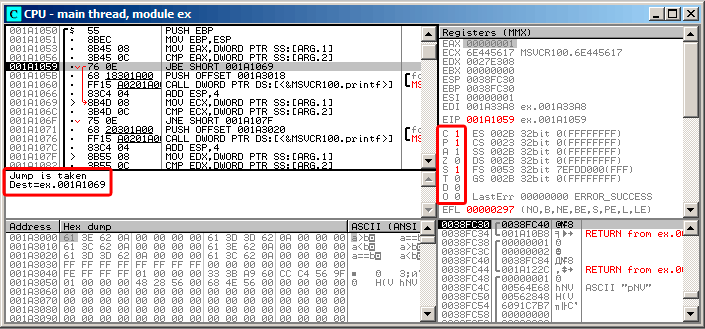
\includegraphics[scale=\FigScale]{patterns/07_jcc/simple/olly_unsigned1.png}
\caption{\olly: \TT{f\_unsigned()}: \RU{первый условный переход}\EN{first conditional jump}}
\label{fig:jcc_olly_unsigned_1}
\end{figure}

\RU{Итак, флаги}\EN{So, the flags are}: C=1, P=1, A=1, Z=0, S=1, T=0, D=0, O=0.
\RU{Для краткости, в \olly флаги называются только одной буквой.}
\EN{They are named with one character for brevity in \olly.}

\olly \RU{подсказывает, что первый переход}\EN{gives a hint that the} (\JBE) 
\RU{сейчас сработает}\EN{jump is to be triggered now}.
\RU{Действительно, если заглянуть в}\EN{Indeed, if we take a look into} \cite{Intel}, 
\RU{прочитаем там, что}
\EN{we can read there that} \JBE \RU{срабатывает в случаях если}\EN{is triggering if} 
CF=1 \OrENRU ZF=1.
\RU{Условие здесь выполняется, так что переход срабатывает}\EN{The condition is true here, so the jump is triggered}.

\clearpage
\RU{Следующий переход}\EN{The next conditional jump}:

\begin{figure}[H]
\centering
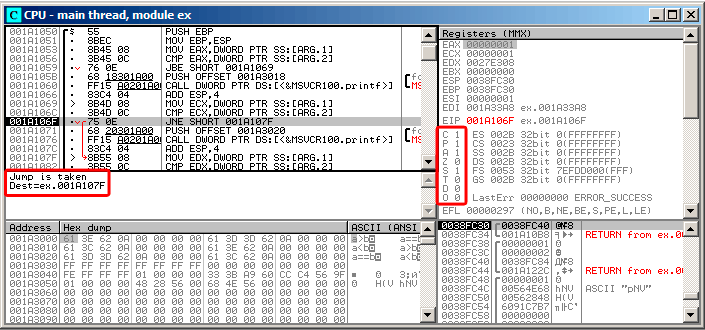
\includegraphics[scale=\FigScale]{patterns/07_jcc/simple/olly_unsigned2.png}
\caption{\olly: \TT{f\_unsigned()}: \RU{второй условный переход}\EN{second conditional jump}}
\label{fig:jcc_olly_unsigned_2}
\end{figure}

\olly \RU{подсказывает, что}\EN{gives a hint that} \JNZ \RU{сработает}\EN{is to be triggered now}.
\RU{Действительно}\EN{Indeed}, \JNZ \RU{срабатывает если}\EN{triggering if} ZF=0 (zero flag).

\clearpage
\RU{Третий переход,}\EN{The third conditional jump,} \JNB:

\begin{figure}[H]
\centering
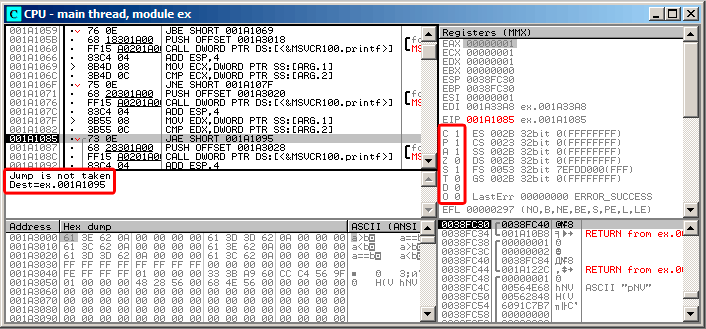
\includegraphics[scale=\FigScale]{patterns/07_jcc/simple/olly_unsigned3.png}
\caption{\olly: \TT{f\_unsigned()}: \RU{третий условный переход}\EN{third conditional jump}}
\label{fig:jcc_olly_unsigned_3}
\end{figure}

\RU{В}\EN{In} \cite{Intel} \RU{мы можем найти, что}\EN{we can see that} \JNB \RU{срабатывает если}
\EN{triggers if} CF=0 (carry flag).
\RU{В нашем случае это не так, переход не срабатывает, и исполняется третий по счету}
\EN{That is not true in our case, so the third} \printf\EN{ will execute}.


\clearpage
\RU{Теперь можно попробовать в \olly функцию}\EN{Now let's review the} \TT{f\_signed()}%
\RU{, работающую с знаковыми величинами}\EN{function, which works with signed values, in \olly}.

\RU{Флаги выставляются точно так же}\EN{Flags are set in the same way}: 
C=1, P=1, A=1, Z=0, S=1, T=0, D=0, O=0.

\RU{Первый переход}\EN{The first conditional jump} \JLE \RU{сработает}\EN{is to be triggered}:

\begin{figure}[H]
\centering
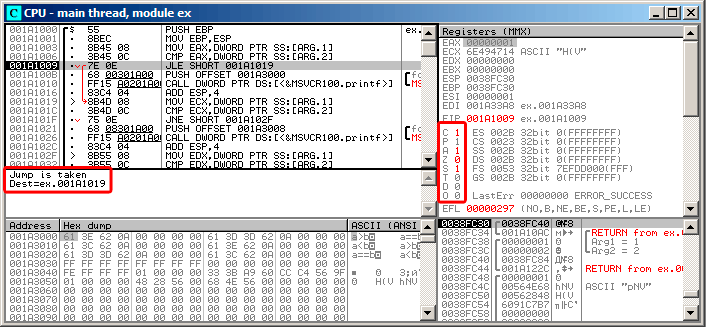
\includegraphics[scale=\FigScale]{patterns/07_jcc/simple/olly_signed1.png}
\caption{\olly: \TT{f\_signed()}: \RU{первый условный переход}\EN{first conditional jump}}
\label{fig:jcc_olly_signed_1}
\end{figure}

\RU{В}\EN{In} \cite{Intel} \RU{мы можем прочитать, что эта инструкция срабатывает если}\EN{we find
that this instruction is triggered if} 
ZF=1 \OrENRU SF$\neq$OF.
\RU{В нашем случае }SF$\neq$OF\RU{, так что переход срабатывает}\EN{ in our case, so the jump triggers}.

\clearpage
\RU{Второй переход}\EN{The second} \JNZ \RU{сработает}\EN{conditional jump triggering}: 
\RU{он срабатывает если}\EN{if} ZF=0 (zero flag):


\begin{figure}[H]
\centering
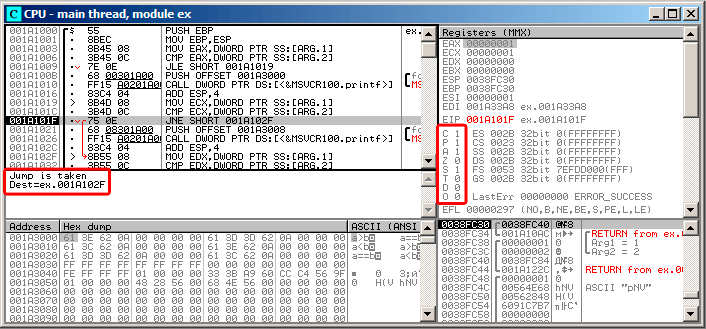
\includegraphics[scale=\FigScale]{patterns/07_jcc/simple/olly_signed2.png}
\caption{\olly: \TT{f\_signed()}: \RU{второй условный переход}\EN{second conditional jump}}
\label{fig:jcc_olly_signed_2}
\end{figure}

\clearpage
\RU{Третий переход}\EN{The third conditional jump} \JGE 
\RU{не сработает, потому что он срабатывает, только если}\EN{will not trigger because it would only do so if} SF=OF, 
\RU{что в нашем случае не так}\EN{and that is not true in our case}:

\begin{figure}[H]
\centering
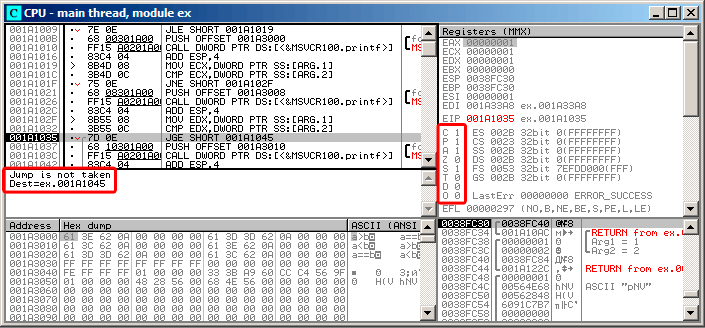
\includegraphics[scale=\FigScale]{patterns/07_jcc/simple/olly_signed3.png}
\caption{\olly: \TT{f\_signed()}: \RU{третий условный переход}\EN{third conditional jump}}
\label{fig:jcc_olly_signed_3}
\end{figure}

\fi

\clearpage
\subsubsection{x86 + MSVC + Hiew}
\index{Hiew}

\RU{Можем попробовать модифицировать исполняемый файл так,}\EN{We can try to patch the executable file in a way} 
\RU{чтобы функция}\EN{that the} \TT{f\_unsigned()} \RU{всегда показывала}\EN{function would always print} \q{a==b}, 
\RU{при любых входящих значениях}\EN{no matter the input values}.
\RU{Вот как она выглядит в}\EN{Here is how it looks in} Hiew:

\begin{figure}[H]
\centering
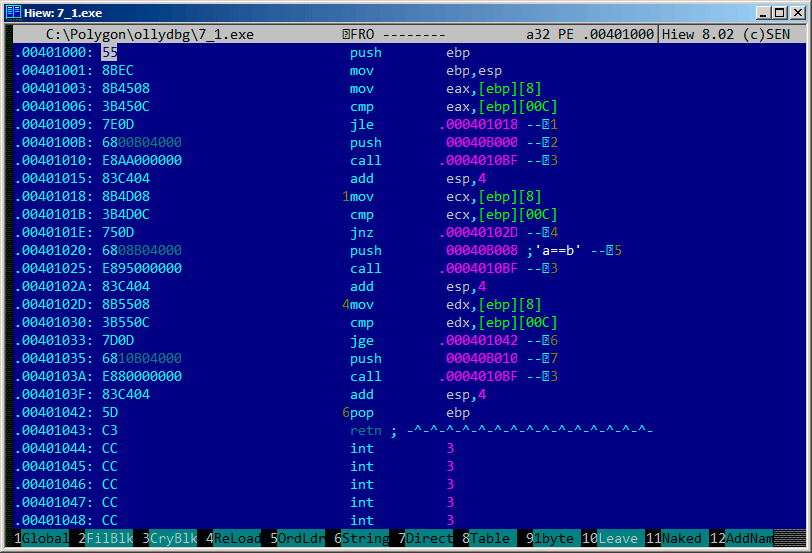
\includegraphics[scale=\FigScale]{patterns/07_jcc/simple/hiew_unsigned1.png}
\caption{Hiew: \RU{функция }\TT{f\_unsigned()}\EN{ function}}
\label{fig:jcc_hiew_1}
\end{figure}

\RU{Собственно, задач три}\EN{Essentially, we need to accomplish three tasks}:
\begin{itemize}
\item \RU{заставить первый переход срабатывать всегда}\EN{force the first jump to always trigger};
\item \RU{заставить второй переход не срабатывать никогда}\EN{force the second jump to never trigger};
\item \RU{заставить третий переход срабатывать всегда}\EN{force the third jump to always trigger}.
\end{itemize}

\RU{Так мы направим путь исполнения кода (code flow) во второй}\EN{Thus we can direct the code flow
to always pass through the second} \printf,
\RU{и он всегда будет срабатывать и выводить на консоль}\EN{and output} \q{a==b}.

\RU{Для этого нужно изменить три инструкции (или байта)}\EN{Three instructions (or bytes) has to be patched}:

\begin{itemize}
\item \RU{Первый переход теперь будет}\EN{The first jump becomes} \JMP, \RU{но смещение перехода 
(\gls{jump offset}) останется прежним}\EN{but the \gls{jump offset} would remain the same}.

\item \RU{Второй переход может быть и будет срабатывать иногда, но в любом случае он будет совершать переход
только на следующую инструкцию, потому что мы выставляем смещение перехода (\gls{jump offset}) в 0.}
\EN{The second jump might be triggered sometimes, but in any case it will jump to the next
instruction, because, we set the \gls{jump offset} to 0.}
\RU{В этих инструкциях смещение перехода просто прибавляется к адресу следующей инструкции.}
\EN{In these instructions the \gls{jump offset} is added to the address for the next instruction.}
\RU{Когда смещение 0, переход будет на следующую инструкцию.}\EN{So if the offset is 0,
the jump will transfer the control to the next instruction.}

\item \RU{Третий переход конвертируем в \JMP точно так же, как и первый, он будет срабатывать всегда.}
\EN{The third jump we replace with \JMP just as we do with the first one, so it will always trigger.}

\end{itemize}

\clearpage
\RU{Что и делаем}\EN{Here is the modified code}:

\begin{figure}[H]
\centering
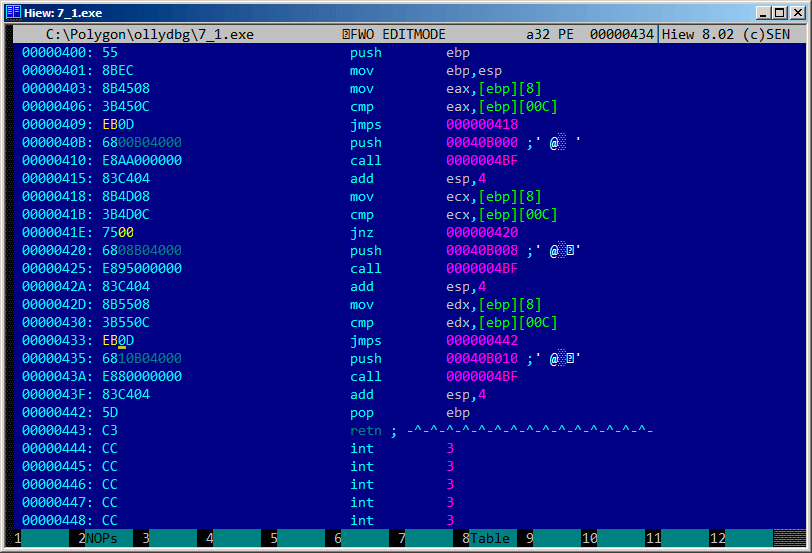
\includegraphics[scale=\FigScale]{patterns/07_jcc/simple/hiew_unsigned2.png}
\caption{Hiew: \RU{модифицируем функцию}\EN{let's modify the} \TT{f\_unsigned()}\EN{ function}}
\label{fig:jcc_hiew_2}
\end{figure}

\RU{Если забыть про какой-то из переходов, то тогда будет срабатывать несколько вызовов \printf, 
а нам ведь нужно чтобы исполнялся только один.}
\EN{If we miss to change any of these jumps, then several \printf calls may execute, while we want to execute only one.}

\ifdefined\IncludeGCC
\subsubsection{\NonOptimizing GCC}

\index{puts() \RU{вместо}\EN{instead of} printf()}
\NonOptimizing GCC 4.4.1 \RU{производит почти такой же код, за исключением}
\EN{produces almost the same code, but with} \puts~(\myref{puts}) \RU{вместо}\EN{instead of} \printf.

\subsubsection{\Optimizing GCC}

\RU{Наблюдательный читатель может спросить, зачем исполнять \CMP так много раз,
если флаги всегда одни и те же}\EN{An observant reader may ask, why execute \CMP several times, 
if the flags has the same values after each execution}?
\RU{По видимому, оптимизирующий MSVC не может этого делать, но GCC 4.8.1 делает больше оптимизаций:}
\EN{Perhaps optimizing MSVC can not do this, but optimizing GCC 4.8.1 can go deeper:}

\lstinputlisting[caption=GCC 4.8.1 f\_signed()]{patterns/07_jcc/simple/GCC_O3_signed.asm}

% should be here instead of 'switch' section?
\RU{Мы здесь также видим}\EN{We also see} \TT{JMP puts} \RU{вместо}\EN{here instead of} \TT{CALL puts / RETN}.
\RU{Этот прием описан немного позже}%
\EN{This kind of trick will have explained later}: \myref{JMP_instead_of_RET}.

\RU{Нужно сказать, что x86-код такого типа редок}\EN{This type of x86 code 
is somewhat rare}.
MSVC 2012\RU{, как видно, не может генерировать подобное}\EN{ as it seems, can't generate such code}.
\RU{С другой стороны, программисты на ассемблере прекрасно осведомлены о том, что инструкции}\EN{On the other hand, assembly language programmers are fully aware of the fact that} \TT{Jcc} \RU{можно располагать последовательно.}
\EN{instructions can be stacked.}
\RU{Так что если вы видите это где-то, имеется немалая вероятность, что этот фрагмент кода был написан вручную.}
\EN{So if you see such stacking somewhere, it is highly probable that the code was hand-written.}

\EN{The}\RU{Функция} \TT{f\_unsigned()} \RU{получилась не настолько эстетически короткой}\EN{function is not that 
\ae{}sthetically short}:

\lstinputlisting[caption=GCC 4.8.1 f\_unsigned()]{patterns/07_jcc/simple/GCC_O3_unsigned.asm.\LANG}

\RU{Тем не менее, здесь 2 инструкции \TT{CMP} вместо трех.}
\EN{Nevertheless, there are two \TT{CMP} instructions instead of three.}
\RU{Так что, алгоритмы оптимизации GCC 4.8.1, наверное, ещё пока не идеальны.}
\EN{So optimization algorithms of GCC 4.8.1 are probably not perfect yet.} 
\fi

\ifdefined\IncludeARM
\subsection{ARM}

% subsubsections here
\subsubsection{32-\RU{битный}\EN{bit} ARM}
\label{subsec:jcc_ARM}

\myparagraph{\OptimizingKeilVI (\ARMMode)}

\lstinputlisting[caption=\OptimizingKeilVI (\ARMMode)]{patterns/07_jcc/simple/ARM/ARM_O3_signed.asm}

\index{ARM!Condition codes}
% FIXME \ref -> which instructions?
\RU{Многие инструкции в режиме ARM могут быть исполнены только при некоторых выставленных флагах.}
\EN{Many instructions in ARM mode could be executed only when specific flags are set.}
\RU{Это нередко используется для сравнения чисел.}
\EN{E.g. this is often used when comparing numbers.}

\index{ARM!\Instructions!ADD}
\index{ARM!\Instructions!ADDAL}
\RU{К примеру, инструкция \ADD на самом деле называется \TT{ADDAL} внутри, \TT{AL} означает 
\IT{Always}, то есть, исполнять всегда.}
\EN{For instance, the \ADD instruction is in fact named \TT{ADDAL} internally, where \TT{AL} stands for
\IT{Always}, i.e., execute always.}
\RU{Предикаты кодируются в 4-х старших битах инструкции 32-битных ARM-инструкций}
\EN{The predicates are encoded in 4 high bits of the 32-bit ARM instructions} (\IT{condition field}).
\index{ARM!\Instructions!B}
\RU{Инструкция безусловного перехода \TT{B} на самом деле условная и кодируется так же, 
как и прочие инструкции условных переходов, но имеет \TT{AL} в \IT{condition field}, 
то есть исполняется всегда (\IT{execute ALways}), игнорируя флаги.}
\EN{The \TT{B} instruction for unconditional jumping is in fact conditional and encoded just like any other
conditional jump, but has \TT{AL} in the \IT{condition field}, and it implies \IT{execute ALways}, 
ignoring flags.}

\index{ARM!\Instructions!ADR}
\index{ARM!\Instructions!ADRcc}
\index{ARM!\Instructions!CMP}
\RU{Инструкция \TT{ADRGT} работает так же, как и \TT{ADR}, но исполняется только в случае,
если предыдущая инструкция \CMP,
сравнивая два числа, обнаруживает, что одно из них больше второго (\IT{Greater Than}).}
\EN{The \TT{ADRGT} instruction works just like \TT{ADR} but executes only in case the previous \CMP
instruction founds one of the numbers greater than the another, while comparing the two (\IT{Greater Than}).}

\index{ARM!\Instructions!BL}
\index{ARM!\Instructions!BLcc}
\RU{Следующая инструкция \TT{BLGT} ведет себя так же, как и \TT{BL} и сработает, только если 
результат сравнения был такой же}
\EN{The next \TT{BLGT} instruction behaves exactly as \TT{BL} 
and is triggered only if the result of the comparison was the same} (\IT{Greater Than}). 
\TT{ADRGT} \RU{записывает в \Reg{0} указатель на строку}\EN{writes a pointer to the string} 
\TT{a>b\textbackslash{}n}
\RU{, а \TT{BLGT} вызывает}\EN{ into \Reg{0} and \TT{BLGT} calls} \printf.
\RU{Следовательно, эти инструкции с суффиксом \TT{-GT} исполнятся только в том случае, если значение
в \Reg{0} (там $a$) было больше, чем значение в \Reg{4} (там $b$).}
\EN{therefore, these instructions with suffix \TT{-GT} are to execute only in case the value in \Reg{0} (which is $a$) is bigger than the value in \Reg{4} (which is $b$).}

\index{ARM!\Instructions!ADRcc}
\index{ARM!\Instructions!BLcc}
\RU{Далее мы увидим инструкции \TT{ADREQ} и \TT{BLEQ}.}
\EN{Moving forward we see the \TT{ADREQ} and \TT{BLEQ} instructions.}
\RU{Они работают так же, как и \TT{ADR} и \TT{BL}, но исполнятся только если значения при последнем сравнении были равны.}
\EN{They behave just like \TT{ADR} and \TT{BL}, but are to be executed only if operands were equal to each
other during the last comparison.}
\RU{Перед ними расположен ещё один \CMP, потому что вызов \printf мог испортить состояние флагов.}
\EN{Another \CMP is located before them (because the \printf execution may have tampered the flags).}

\index{ARM!\Instructions!LDMccFD}
\index{ARM!\Instructions!LDMFD}
\RU{Далее мы увидим \TT{LDMGEFD}. Эта инструкция работает так же, как и \TT{LDMFD}\footnote{\ac{LDMFD}}, 
но сработает только если в результате сравнения одно из значений было больше или равно второму}
\EN{Then we see \TT{LDMGEFD}, this instruction works just like \TT{LDMFD}\footnote{\ac{LDMFD}},
but is triggered only when one of the values is greater or equal than the other}
(\IT{Greater or Equal}).


\RU{Смысл инструкции}\EN{The } \TT{LDMGEFD SP!, \{R4-R6,PC\}} 
\RU{в том, что это как бы эпилог функции, но он сработает только если $a>=b$, только тогда работа 
функции закончится.}
\EN{instruction acts like a function epilogue, but it will be triggered only if $a>=b$, and only then the function execution will finish.}

\index{Function epilogue}
\RU{Но если это не так, то есть $a<b$, то исполнение дойдет до следующей инструкции 
\TT{LDMFD SP!, \{R4-R6,LR\}}. Это ещё один эпилог функции. Эта инструкция восстанавливает состояние регистров
\TT{R4-R6}, но и \ac{LR} вместо \ac{PC}, таким образом, пока что, не делая возврата из функции.}
\EN{But if that condition is not satisfied, i.e., $a<b$, then the control flow will continue to the next \TT{\q{LDMFD SP!, \{R4-R6,LR\}}} instruction, which is one more function epilogue. This instruction restores not only the \TT{R4-R6} registers state, but also \ac{LR} instead of \ac{PC}, thus, it does not returns from the function.}

\RU{Последние две инструкции вызывают}\EN{The last two instructions call} \printf 
\RU{со строкой}\EN{with the string} <<a<b\textbackslash{}n>> \RU{в качестве единственного аргумента}\EN{as 
a sole argument}.
\RU{Безусловный переход на \printf вместо возврата из функции мы уже рассматривали в секции}
\EN{We already examined an unconditional jump to the \printf function instead of function return in} <<\PrintfSeveralArgumentsSectionName>>\EN{ section}~(\myref{ARM_B_to_printf}).

\index{ARM!\Instructions!ADRcc}
\index{ARM!\Instructions!BLcc}
\index{ARM!\Instructions!LDMccFD}
\RU{Функция }\TT{f\_unsigned} \RU{точно такая же, но там используются инструкции}\EN{is similar,
only the} \TT{ADRHI}, \TT{BLHI}, \AndENRU \TT{LDMCSFD}\RU{. Эти предикаты}\EN{ instructions are
used there, these predicates}
(\IT{HI = Unsigned higher, CS = Carry Set (greater than or equal)}) 
\RU{аналогичны рассмотренным, но служат для работы с беззнаковыми значениями.}
\EN{are analogous to those examined before, but for unsigned values.}

\RU{В функции \main ничего нового для нас нет:}
\EN{There is not much new in the \main function for us:}
\lstinputlisting[caption=\main]{patterns/07_jcc/simple/ARM/ARM_O3_main.asm}

\RU{Так, в режиме ARM можно обойтись без условных переходов.}
\EN{That is how you can get rid of conditional jumps in ARM mode.}

\index{\RU{Конвейер RISC}\EN{RISC pipeline}}
\RU{Почему это хорошо?}\EN{Why is this so good?} \RU{Читайте здесь}\EN{Read here}: \myref{branch_predictors}.

\index{x86!\Instructions!CMOVcc}
\RU{В x86 нет аналогичной возможности, если не считать инструкцию \TT{CMOVcc}, это то же что и \MOV, 
но она срабатывает
только при определенных выставленных флагах, обычно выставленных при помощи \CMP во время сравнения.}
\EN{There is no such feature in x86, except the \TT{CMOVcc} instruction, it is the same as \MOV,
but triggered only when specific flags are set, usually set by \CMP.}

\myparagraph{\OptimizingKeilVI (\ThumbMode)}

\lstinputlisting[caption=\OptimizingKeilVI (\ThumbMode)]{patterns/07_jcc/simple/ARM/ARM_thumb_signed.asm}

\index{ARM!\Instructions!BLE}
\index{ARM!\Instructions!BNE}
\index{ARM!\Instructions!BGE}
\index{ARM!\Instructions!BLS}
\index{ARM!\Instructions!BCS}
\index{ARM!\Instructions!B}
\index{ARM!\ThumbMode}
\RU{В режиме Thumb только инструкции \TT{B} могут быть дополнены условием исполнения (\IT{condition code}), 
так что код для режима Thumb выглядит привычнее.}
\EN{Only \TT{B} instructions in Thumb mode may be supplemented by \IT{condition codes}, so the Thumb code 
looks more ordinary.}

\TT{BLE} \RU{это обычный переход с условием}\EN{is a normal conditional jump} \IT{Less than or Equal}, 
\TT{BNE}\EMDASH\IT{Not Equal}, 
\TT{BGE}\EMDASH\IT{Greater than or Equal}.

\RU{Функция }\TT{f\_unsigned} \RU{точно такая же, но для работы с беззнаковыми величинами 
там используются инструкции}\EN{is similar, only other instructions are used while dealing 
with unsigned values:} \TT{BLS} 
(\IT{Unsigned lower or same}) \AndENRU \TT{BCS} (\IT{Carry Set (Greater than or equal)}).

\subsubsection{ARM64: \Optimizing GCC (Linaro) 4.9}

\lstinputlisting[caption=f\_signed()]{patterns/07_jcc/simple/ARM/ARM64_GCC_O3_signed.lst.\LANG}

\lstinputlisting[caption=f\_unsigned()]{patterns/07_jcc/simple/ARM/ARM64_GCC_O3_unsigned.lst.\LANG}

\EN{The comments were added by the author of this book}\RU{Комментарии добавлены автором этой книги}.
\EN{What is striking is that the compiler is not aware that some conditions are not possible at all,
so there is dead code at some places, which can never be executed.}
\RU{В глаза бросается то, что компилятор не в курсе, что некоторые ситуации невозможны,
поэтому кое-где в функциях остается код, который никогда не исполнится.}

\myparagraph{\Exercise}

\EN{Try to optimize these functions manually for size, removing redundant instructions, without adding new ones.}
\RU{Попробуйте вручную оптимизировать функции по размеру, убрав избыточные инструкции и не добавляя новых.}


\fi
\ifdefined\IncludeMIPS
\subsection{MIPS}

\RU{Одна отличительная особенность MIPS это отсутствие регистра флагов.}
\EN{One distinctive MIPS feature is the absence of flags.}
\RU{Очевидно, так было сделано для упрощения анализа зависимости данных (data dependency).}
\EN{Apparently, it was done to simplify the analysis of data dependencies.}

\index{x86!\Instructions!SETcc}
\index{MIPS!\Instructions!SLT}
\index{MIPS!\Instructions!SLTU}
\RU{Так что здесь есть инструкция, похожая на SETcc в x86: SLT (\q{Set on Less Than}~--- установить если
меньше чем, знаковая версия) и SLTU (беззнаковая версия).}
\EN{There are instructions similar to SETcc in x86: SLT (\q{Set on Less Than}: signed version) and 
SLTU (unsigned version).}
\RU{Эта инструкция устанавливает регистр-получатель в 1 если условие верно или в 0 в противном случае.}
\EN{These instructions sets destination register value to 1 if the condition is true or to 0 if otherwise.}

\index{MIPS!\Instructions!BEQ}
\index{MIPS!\Instructions!BNE}
\RU{Затем регистр-получатель проверяется, используя инструкцию 
BEQ (\q{Branch on Equal} --- переход если равно) или BNE (\q{Branch on Not Equal} --- переход если не равно) 
и может произойти переход.}
\EN{The destination register is then checked using BEQ (\q{Branch on Equal}) or BNE (\q{Branch on Not Equal}) 
and a jump may occur.}

\RU{Так что эта пара инструкций должна использоваться в MIPS для сравнения и перехода.}
\EN{So, this instruction pair has to be used in MIPS for comparison and branch.}

\RU{Начнем с знаковой версии нашей функции:}
\EN{Let's first start with the signed version of our function:}

\lstinputlisting[caption=\NonOptimizing GCC 4.4.5 (IDA)]{patterns/07_jcc/simple/O0_MIPS_signed_IDA.lst.\LANG}

\q{SLT REG0, REG0, REG1} \RU{сокращается в IDA до более короткой формы}\EN{is reduced by IDA to its 
shorter form} \q{SLT REG0, REG1}.
\index{MIPS!\Pseudoinstructions!BEQZ}
\RU{Мы также видим здесь псевдоинструкцию BEQZ (\q{Branch if Equal to Zero}~--- переход если равно нулю), 
которая, на самом деле, \q{BEQ REG, \$ZERO, LABEL}.}
\EN{We also see there BEQZ pseudoinstruction (\q{Branch if Equal to Zero}), 
which are in fact \q{BEQ REG, \$ZERO, LABEL}.}

\index{MIPS!\Instructions!SLTU}
\RU{Беззнаковая версия точно такая же, только здесь используется SLTU (беззнаковая версия, 
отсюда \q{U} в названии) вместо SLT:}
\EN{The unsigned version is just the same, but SLTU (unsigned version, hence \q{U} in name) is used instead of SLT:}

\lstinputlisting[caption=\NonOptimizing GCC 4.4.5 (IDA)]{patterns/07_jcc/simple/O0_MIPS_unsigned_IDA.lst}

\fi

\section{\RU{Вычисление абсолютной величины}\EN{Calculating absolute value}}
\label{sec:abs}

\RU{Это простая функция}\EN{A simple function}:

\lstinputlisting{abs.c}

\subsection{\Optimizing MSVC}

\RU{Обычный способ генерации кода:}
\EN{This is how the code is usually generated:}

\lstinputlisting[caption=\Optimizing MSVC 2012 x64]{patterns/07_jcc/abs/abs_MSVC2012_Ox_x64.asm.\LANG}

\ifdefined\IncludeGCC
\RU{GCC 4.9 делает почти то же самое.}
\EN{GCC 4.9 does mostly the same.}
\fi

\ifdefined\IncludeARM
\subsection{\OptimizingKeilVI: \ThumbMode}

\lstinputlisting[caption=\OptimizingKeilVI: \ThumbMode]{patterns/07_jcc/abs/abs_Keil_thumb_O3.s.\LANG}

\index{ARM!\Instructions!RSB}
\RU{В ARM нет инструкции для изменения знака, так что компилятор Keil использует инструкцию \q{Reverse Subtract},
которая просто вычитает, но с операндами, переставленными наоборот.}
\EN{ARM lacks a negate instruction, so the Keil compiler uses the \q{Reverse Subtract} instruction, which just subtracts with reversed operands.}

\subsection{\OptimizingKeilVI: \ARMMode}

\RU{В режиме ARM можно добавлять коды условий к некоторым инструкций, что компилятор Keil и сделал:}
\EN{It is possible to add condition codes to some instructions in ARM mode, so that is what the Keil compiler does:}

\lstinputlisting[caption=\OptimizingKeilVI: \ARMMode]{patterns/07_jcc/abs/abs_Keil_ARM_O3.s.\LANG}

\RU{Теперь здесь нет условных переходов и это хорошо:}
\EN{Now there are no conditional jumps and this is good:} 
\myref{branch_predictors}.

\subsection{\NonOptimizing GCC 4.9 (ARM64)}

\index{ARM!\Instructions!XOR}
\RU{В ARM64 есть инструкция NEG для смены знака:}
\EN{ARM64 has instruction NEG for negating:}

\lstinputlisting[caption=\Optimizing GCC 4.9 (ARM64)]{patterns/07_jcc/abs/abs_GCC49_ARM64_O0.s.\LANG}
\fi

\ifdefined\IncludeMIPS
\subsection{MIPS}

\lstinputlisting[caption=\Optimizing GCC 4.4.5 (IDA)]{patterns/07_jcc/abs/MIPS_O3_IDA.lst.\LANG}

\index{MIPS!\Instructions!BLTZ}
\RU{Видим здесь новую инструкцию}\EN{Here we see a new instruction}: BLTZ (\q{Branch if Less Than Zero}).
\index{MIPS!\Instructions!SUBU}
\index{MIPS!\Pseudoinstructions!NEGU}
\RU{Тут есть также псевдоинструкция NEGU, которая на самом деле вычитает из нуля.}
\EN{There is also the NEGU pseudoinstruction, which just does subtraction from zero.}
\RU{Суффикс \q{U} в обоих инструкциях SUBU и NEGU означает, что при целочисленном переполнении исключение не
сработает.}
\EN{The \q{U} suffix in both SUBU and NEGU implies that no exception to be raised in case of integer overflow.}

\fi

\ifx\LITE\undefined
\subsection{\RU{Версия без переходов}\EN{Branchless version}?}

\RU{Возможна также версия и без переходов, мы рассмотрим её позже:}
\EN{You could have also a branchless version of this code. This we will review later:} \myref{chap:branchless_abs}.
\fi

\section{\RU{Тернарный условный оператор}\EN{Ternary conditional operator}}
\label{chap:cond}

\RU{Тернарный условный оператор (ternary conditional operator) в}\EN{The ternary conditional operator in} \CCpp \RU{это}\EN{has the following syntax}:

\begin{lstlisting}
expression ? expression : expression
\end{lstlisting}

\RU{И вот пример}\EN{Here is an example}:

\lstinputlisting{patterns/07_jcc/cond_operator/cond.c}

\subsection{x86}

\RU{Старые и неоптимизирующие компиляторы генерируют код так, как если бы выражение \TT{if/else} было использовано
вместо него:}
\EN{Old and non-optimizing compilers generate assembly code just as if an \TT{if/else} statement was used:}

\lstinputlisting[caption=\NonOptimizing MSVC 2008]{patterns/07_jcc/cond_operator/MSVC2008.asm.\LANG}

\lstinputlisting[caption=\Optimizing MSVC 2008]{patterns/07_jcc/cond_operator/MSVC2008_Ox.asm.\LANG}

\RU{Новые компиляторы могут быть более краткими}\EN{Newer compilers are more concise}:

\lstinputlisting[caption=\Optimizing MSVC 2012 x64]{patterns/07_jcc/cond_operator/MSVC2012_Ox_x64.asm.\LANG}

\index{x86!\Instructions!CMOVcc}
\Optimizing GCC 4.8 \ForENRU x86 \RU{также использует инструкцию}\EN{also uses the} \TT{CMOVcc}\RU{, тогда как
неоптимизирующий GCC 4.8 использует условные переходы}\EN{ instruction, while the non-optimizing GCC 4.8 uses conditional jumps}.

\ifdefined\IncludeARM
\subsection{ARM}

\index{x86!\Instructions!ADRcc}
\Optimizing Keil \ForENRU \RU{режима ARM также использует инструкцию \TT{ADRcc}, срабатывающую при некотором
условии}\EN{ARM mode also uses the conditional instructions \TT{ADRcc}}:

\lstinputlisting[label=cond_Keil_ARM_O3,caption=\OptimizingKeilVI (\ARMMode)]{patterns/07_jcc/cond_operator/Keil_ARM_O3.s.\LANG}

\RU{Без внешнего вмешательства инструкции \TT{ADREQ} и \TT{ADRNE} никогда не исполнятся одновременно.}
\EN{Without manual intervention, the two instructions \TT{ADREQ} and \TT{ADRNE} cannot be executed in the same run.}

\Optimizing Keil \ForENRU \RU{режима Thumb вынужден использовать инструкции условного перехода, потому
что тут нет инструкции загрузки значения, поддерживающей флаги условия}\EN{Thumb mode needs to use 
conditional jump instructions, since there are no load instructions
that support conditional flags}:

\lstinputlisting[caption=\OptimizingKeilVI (\ThumbMode)]{patterns/07_jcc/cond_operator/Keil_thumb_O3.s.\LANG}

\subsection{ARM64}

\Optimizing GCC (Linaro) 4.9 \ForENRU ARM64 \RU{также использует условные переходы}\EN{also uses conditional jumps}:

\lstinputlisting[label=cond_ARM64,caption=\Optimizing GCC (Linaro) 4.9]{patterns/07_jcc/cond_operator/ARM64_GCC_O3.s.\LANG}

\RU{Это потому что в ARM64 нет простой инструкции загрузки с флагами условия, как \TT{ADRcc} в 32-битном 
режиме ARM или \TT{CMOVcc} в x86}
\EN{That is because ARM64 does not have a simple load instruction with conditional flags, like \TT{ADRcc} in 32-bit ARM mode or CMOVcc in x86}
\cite[p390, C5.5]{ARM64ref}.
\index{ARM!\Instructions!CSEL}
\RU{Но с другой стороны, там есть инструкция \TT{CSEL} (\q{Conditional SELect}), но GCC 4.9 наверное, пока не так
хорош, чтобы генерировать её в таком фрагменте кода.}
\EN{It has, however, \q{Conditional SELect} instruction (\TT{CSEL}), but GCC 4.9 does not seem to be smart enough to use it in such piece of code.}
\fi

\ifdefined\IncludeMIPS
\subsection{MIPS}

\RU{GCC 4.4.5 для MIPS тоже не так хорош, к сожалению}\EN{Unfortunately, GCC 4.4.5 for MIPS is not very smart, either}:

\lstinputlisting[caption=\Optimizing GCC 4.4.5 (\assemblyOutput)]{patterns/07_jcc/cond_operator/MIPS_O3.s.\LANG}

\fi

\subsection{\RU{Перепишем, используя обычный \TT{if/else}}\EN{Let's rewrite it in an \TT{if/else} way}}

\lstinputlisting{patterns/07_jcc/cond_operator/cond2.c}

\index{x86!\Instructions!CMOVcc}
\RU{Интересно, оптимизирующий GCC 4.8 для x86 также может генерировать \TT{CMOVcc} в этом случае:}
\EN{Interestingly, optimizing GCC 4.8 for x86 was also able to use \TT{CMOVcc} in this case:}

\lstinputlisting[caption=\Optimizing GCC 4.8]{patterns/07_jcc/cond_operator/cond2_GCC_O3.s.\LANG}

\ifdefined\IncludeARM
\Optimizing Keil \InENRU \RU{режиме ARM генерирует код идентичный этому:}\EN{ARM mode generates 
code identical to} \lstref{cond_Keil_ARM_O3}.
\fi

\RU{Но оптимизирующий}\EN{But the optimizing} MSVC 2012 \RU{пока не так хорош}\EN{is not that good (yet)}.

\ifx\LITE\undefined
\subsection{\Conclusion{}}

\RU{Почему оптимизирующие компиляторы стараются избавиться от условных переходов? Читайте больше об этом здесь:}
\EN{Why optimizing compilers try to get rid of conditional jumps? Read here about it:} \myref{branch_predictors}.
\fi

\section{\RU{Поиск минимального и максимального значения}\EN{Getting minimal and maximal values}}

\subsection{32-bit}

\lstinputlisting{patterns/07_jcc/minmax/minmax.c}

\lstinputlisting[caption=\NonOptimizing MSVC 2013]{patterns/07_jcc/minmax/minmax_MSVC_2013.asm.\LANG}

\index{x86!\Instructions!Jcc}
\RU{Эти две функции отличаются друг от друга только инструкцией условного перехода:
JGE (\q{Jump if Greater or Equal}~--- переход если больше или равно) используется в первой
и JLE (\q{Jump if Less or Equal}~--- переход если меньше или равно) во второй.}
\EN{These two functions differ only in the conditional jump instruction: 
JGE (\q{Jump if Greater or Equal}) is used in the first one
and JLE (\q{Jump if Less or Equal}) in the second.}

\index{\CompilerAnomaly}
\label{MSVC_double_JMP_anomaly}
\RU{Здесь есть ненужная инструкция \JMP в каждой функции, которую MSVC, наверное, оставил по ошибке.}
\EN{There is one unneeded \JMP instruction in each function, which MSVC probably left by mistake.}

\ifx\LITE\undefined
\subsubsection{\RU{Без переходов}\EN{Branchless}}

\RU{ARM в режиме Thumb напоминает нам x86-код:}
\EN{ARM for Thumb mode reminds us of x86 code:}

\lstinputlisting[caption=\OptimizingKeilVI (\ThumbMode)]{patterns/07_jcc/minmax/minmax_Keil_Thumb_O3.s.\LANG}

\index{ARM!\Instructions!Bcc}
\RU{Функции отличаются только инструкцией перехода: BGT и BLT.}
\EN{The functions differ in the branching instruction: BGT and BLT.}

\RU{А в режиме ARM можно использовать условные суффиксы, так что код более плотный.}
\EN{It's possible to use conditional suffixes in ARM mode, so the code is shorter.}
\RU{MOVcc будет исполнена только если условие верно:}
\EN{MOVcc is to be executed only if the condition is met:}
\index{ARM!\Instructions!MOVcc}

\lstinputlisting[caption=\OptimizingKeilVI (\ARMMode)]{patterns/07_jcc/minmax/minmax_Keil_ARM_O3.s.\LANG}

\index{x86!\Instructions!CMOVcc}
\Optimizing GCC 4.8.1 \RU{и оптимизирующий}\EN{and optimizing} MSVC 2013 
\RU{могут использовать инструкцию CMOVcc, которая аналогична MOVcc в ARM:}
\EN{can use CMOVcc instruction, which is analogous to MOVcc in ARM:}

\lstinputlisting[caption=\Optimizing MSVC 2013]{patterns/07_jcc/minmax/minmax_GCC481_O3.s.\LANG}

\subsection{64-bit}

\lstinputlisting{patterns/07_jcc/minmax/minmax64.c}

\RU{Тут есть ненужные перетасовки значений, но код в целом понятен:}
\EN{There is some unneeded value shuffling, but the code is comprehensible:}

\lstinputlisting[caption=\NonOptimizing GCC 4.9.1 ARM64]{patterns/07_jcc/minmax/minmax64_GCC_49_ARM64_O0.s}

\subsubsection{\RU{Без переходов}\EN{Branchless}}

\RU{Нет нужды загружать аргументы функции из стека, они уже в регистрах:}
\EN{No need to load function arguments from the stack, as they are already in the registers:}

\lstinputlisting[caption=\Optimizing GCC 4.9.1 x64]{patterns/07_jcc/minmax/minmax64_GCC_49_x64_O3.s.\LANG}

MSVC 2013 \RU{делает то же самое}\EN{does almost the same}.

\index{ARM!\Instructions!CSEL}
\RU{В ARM64 есть инструкция CSEL, которая работает точно также, как и MOVcc в ARM и CMOVcc в x86, но название
другое:}
\EN{ARM64 has the CSEL instruction, which works just as MOVcc in ARM or CMOVcc in x86, just the name is different:}
\q{Conditional SELect}.

\lstinputlisting[caption=\Optimizing GCC 4.9.1 ARM64]{patterns/07_jcc/minmax/minmax64_GCC_49_ARM64_O3.s.\LANG}

\ifdefined\IncludeMIPS
\subsection{MIPS}

\RU{А GCC 4.4.5 для MIPS не так хорош, к сожалению}\EN{Unfortunately, GCC 4.4.5 for MIPS is not that good}:

\lstinputlisting[caption=\Optimizing GCC 4.4.5 (IDA)]{patterns/07_jcc/minmax/minmax_MIPS_O3_IDA.lst.\LANG}

\RU{Не забывайте о \IT{branch delay slots}: первая MOVE исполняется \IT{перед} BEQZ,
вторая MOVE исполняется только если переход не произошел.}
\EN{Do not forget about the \IT{branch delay slots}: the first MOVE is executed \IT{before} BEQZ, 
the second MOVE is executed only if the branch wasn't taken.}

\fi
\fi


\section{\Conclusion{}}

\subsection{x86}

\RU{Примерный скелет условных переходов}\EN{Here's the rough skeleton of a conditional jump}:

\lstinputlisting[caption=x86]{patterns/07_jcc/skel1.lst.\LANG}

\ifdefined\IncludeARM

\subsection{ARM}

\lstinputlisting[caption=ARM]{patterns/07_jcc/skel2.lst.\LANG}
\fi

\ifdefined\IncludeMIPS

\subsection{MIPS}

\begin{lstlisting}[caption=\RU{Проверка на ноль}\EN{Check for zero}]
BEQZ REG, label
...
\end{lstlisting}

\begin{lstlisting}[caption=\RU{Меньше ли нуля?}\EN{Check for less than zero:}]
BLTZ REG, label
...
\end{lstlisting}

\begin{lstlisting}[caption=\RU{Проверка на равенство}\EN{Check for equal values}]
BEQ REG1, REG2, label
...
\end{lstlisting}

\begin{lstlisting}[caption=\RU{Проверка на неравенство}\EN{Check for non-equal values}]
BNE REG1, REG2, label
...
\end{lstlisting}

\begin{lstlisting}[caption=\RU{Проверка на меньше, больше (знаковое)}\EN{Check for less than, greater than (signed)}]
SLT REG1, REG2, REG3
BEQ REG1, label
...
\end{lstlisting}

\begin{lstlisting}[caption=\RU{Проверка на меньше, больше (беззнаковое)}\EN{Check for less than, greater than (unsigned)}]
SLTU REG1, REG2, REG3
BEQ REG1, label
...
\end{lstlisting}
\fi

\subsection{\RU{Без инструкций перехода}\EN{Branchless}}

\index{ARM!\Instructions!MOVcc}
\index{x86!\Instructions!CMOVcc}
\index{ARM!\Instructions!CSEL}
\EN{If the body of a condition statement is very short, the conditional move instruction can be used: 
MOVcc in ARM (in ARM mode), CSEL in ARM64, CMOVcc in x86.}
\RU{Если тело условного выражения очень короткое, может быть
использована инструкция условного копирования: MOVcc в ARM (в режиме ARM), CSEL в ARM64, CMOVcc в x86.}

\ifdefined\IncludeARM
\subsubsection{ARM}

\RU{В режиме ARM можно использовать условные суффиксы для некоторых инструкций:}
\EN{It's possible to use conditional suffixes in ARM mode for some instructions:}

\lstinputlisting[caption=ARM (\ARMMode)]{patterns/07_jcc/skel4.lst.\LANG}

\RU{Нет никаких ограничений на количество инструкций с условными суффиксами до тех пор,
пока флаги CPU не были модифицированы одной из таких инструкций.}
\EN{Of course, there is no limit for the number of instructions with conditional code suffixes, 
as long as the CPU flags are not modified by any of them.}
% FIXME: list of such instructions or \myref{} to it

\index{ARM!\Instructions!IT}
\RU{В режиме Thumb есть инструкция IT, позволяющая дополнить следующие 4 инструкции суффиксами, задающими
условие.}
\EN{Thumb mode has the IT instruction, allowing to add conditional suffixes to the next four instructions.}
\RU{Читайте больше об этом}\EN{Read more about it}: \myref{ARM_Thumb_IT}.

\lstinputlisting[caption=ARM (\ThumbMode)]{patterns/07_jcc/skel3.lst.\LANG}
\fi

\ifdefined\IncludeExercises
\section{\Exercise}

(ARM64) \RU{Попробуйте переписать код в}\EN{Try rewriting the code in} \lstref{cond_ARM64} 
\RU{убрав все инструкции условного перехода, и используйте инструкцию \TT{CSEL}}\EN{by removing all 
conditional jump instructions and using the \TT{CSEL} instruction}.
\fi

